\documentclass{jps-cp}
\usepackage{txfonts} %Please comment out this line unless the txfonts package is availabe in your LaTeX system.
\usepackage{url}
\usepackage{multirow}
\usepackage{array, booktabs}
\usepackage{wrapfig}

\makeatletter
\newcommand{\figcaption}[1]{\def\@captype{figure}\caption{#1}}
\newcommand{\tblcaption}[1]{\def\@captype{table}\caption{#1}}

\title{New analysis method of TPC data using neural network}

\author{
  Takanobu \textsc{Doi}$^{1}$, Takahiro \textsc{Kawabata}$^{2}$, Tatsuya \textsc{Furuno}$^{3}$,
  Yuki \textsc{Fujikawa}$^{1}$, Kento \textsc{Inaba}$^{1}$, Motoki \textsc{Murata}$^{3}$,
  Shintaro \textsc{Okamoto}$^{1}$ and Akane \textsc{Sakaue}$^{1}$}

\inst{
  $^{1}$Department of Physics, Kyoto University, Kyoto, Kyoto 606-8502, Japan \\
  $^{2}$Department of Physics, Osaka University, Toyonaka, Osaka 540-0043, Japan \\
  $^{3}$Research Center for Nuclear Physics, Osaka University, Ibaraki, Osaka 567-0047, Japan }

\email{doi.takanobu.68x@st.kyoto-u.ac.jp}

\recdate{2019/8/4} % Write received date here

\abst{
  TPC を用いた実験では荷電粒子の奇跡を3次元的に測定することができる。
  従来はHough 変換を用いてデータの解析を行って来た。
  この方法を用いた解析には多くの労力を要する。
  近年、画像データの認識にはニューラルネットワークが注目されている。
  本研究では、新しくニューラルネットワークを用いた解析方法の開発を行った。
  新しく開発した手法を用いることで、従来の方法と比較して高速に解析できるようになった。
} % Write abstract here

\kword{neural networks, convolutional neural networks,
  TPC, active target, MAIKo TPC} % Write keywords here

\begin{document}
\maketitle

\section{Introduction}
近年、不安定核を用いた原子核実験において検出ガスを標的として用いるアクティブ標的が多く用いられている。
また、荷電粒子の飛跡を2次元的に検出することができるTime Projection Chamber (TPC) が多く用いられている。
TPC は大きな立体角を覆うことができ、多くの物理量を同時に測定することが可能である。
このアクティブ標的を用いたTPC のデータ解析において、
背景事象となるデータの選別や飛跡データの物理的情報の抽出には多くの労力が必要となる。
そこで、我々は近年画像認識において多くの成果を出しているニューラルネットワークを用いることで、
より効率的な解析を行うことができる解析方法の開発を行った。

\section{What is MAIKo TPC}

\begin{wrapfigure}{r}{15zw}
  \begin{center}
    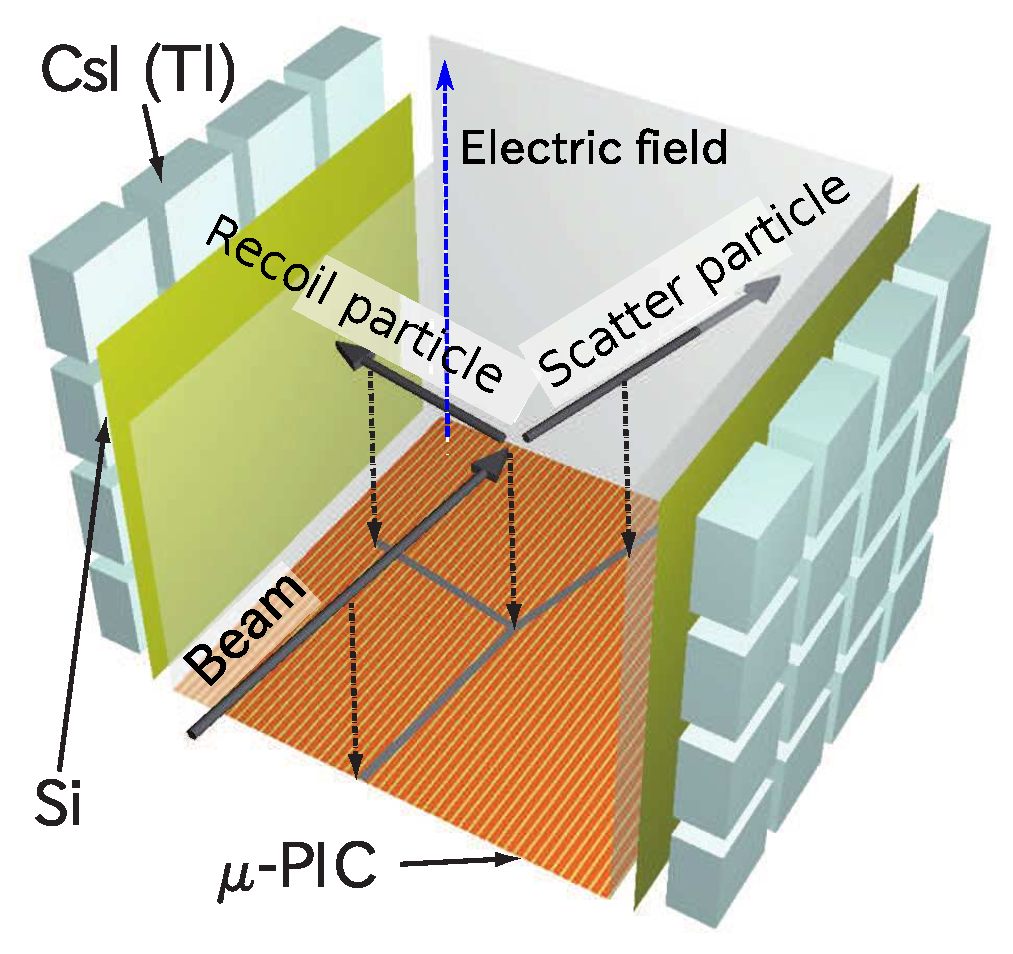
\includegraphics[clip, width=0.4\columnwidth]{eps/at_fig2.eps}
    \caption{MAIKo TPC の外観。}
    \label{fig:MAIKo}
  \end{center}
\end{wrapfigure}

我々は不安定核実験に用いるためにMicro Pixel Chamber ($\mu$-PIC)~\cite{mupic} 
で読み出しを行うTPC とアクティブ標的を用いた検出器である
Mu-Pic based Active target for Inverse Kinematics . (MAIKo) TPC~\cite{MAIKo} (Fig. \ref{fig:MAIKo}) を
不安定核実験に用いるために開発した。
MAIKo TPC の大きさは$102.4 \rm{mm} (\rm{W}) \times 102.4 \rm{mm} (\rm{D}) \times 140.0 \rm{mm} (\rm{H})$である。
MAIKo TPC では飛跡を3次元情報として取得せず、側面方向とビーム入射方向の2つの平面へ射影した飛跡として得られる。
それぞれの画像は$256\times 1024$ pixelsで得られる。

近年、大阪大学核物理研究センター (RCNP) において、
MAIKo TPC を用いた${}^{10}\rm{C}$と${}^{4}\rm{He}$の非弾性散乱の測定が初めて行われた。
MAIKo TPC からはFig. \ref{fig:true}, \ref{fig:false}に示すような飛跡データが得られる。
各図ともに左図が側面に射影した飛跡、右図がビーム方向に射影した飛跡を示す。
MAIKo TPC では標的である${}^{4}\rm{He}$との散乱事象以外にもクエンチガスの$\rm{C}$や$\rm{O}$との散乱も測定される。
飛跡情報の抽出を行うためには背景事象と標的との散乱事象との識別を行わなければならない。
その後に飛跡の長さや方向などの物理的情報の抽出を行う。

\begin{figure}
  \centering
  \begin{minipage}{0.4\columnwidth}
    \centering
    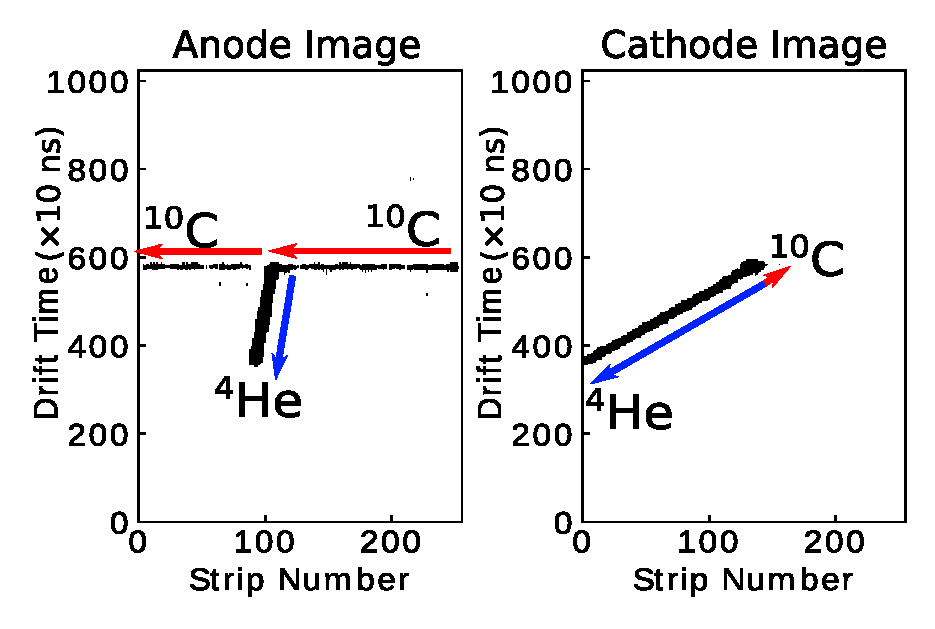
\includegraphics[clip, width=0.9\columnwidth]{eps/true.eps}
    \caption{${}^{10}\rm{C}+{}^{4}\rm{He}$の散乱事象}
    \label{fig:true}
  \end{minipage}
  \begin{minipage}{0.4\columnwidth}
    \centering
    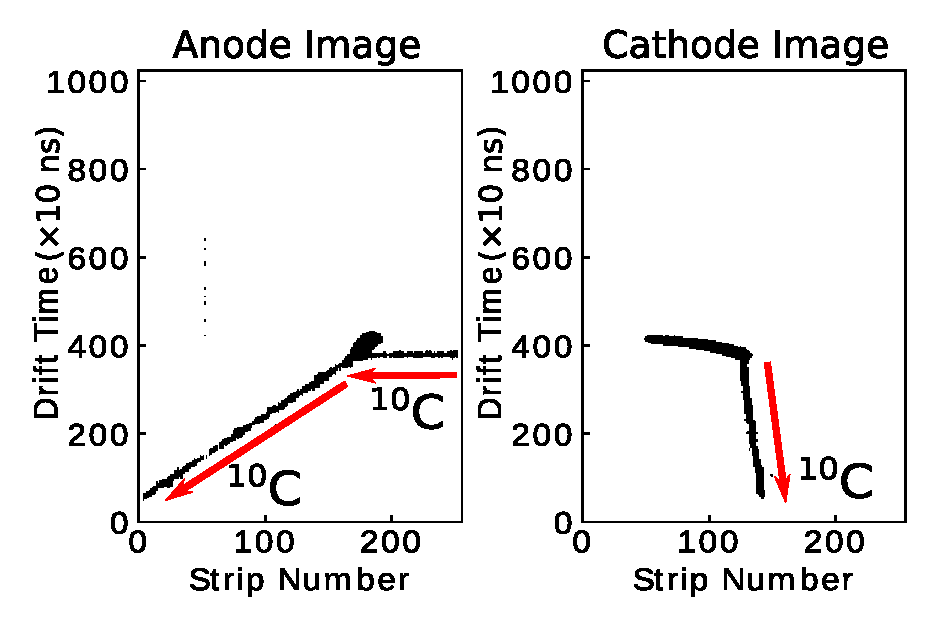
\includegraphics[clip, width=0.9\columnwidth]{eps/false.eps}
    \caption{${}^{10}\rm{C}$とクエンチガスとの散乱事象}
    \label{fig:false}
  \end{minipage}
\end{figure}

\section{Conventional analysis method}
従来は、MAIKo TPC から得られるデータから背景事象の除去を画像から直線を抽出する方法の1つである
Hough 変換を用いたアルゴリズムによって行ってきた。
Hough 変換を行うことで画像は、原点からの距離 ($r$) と傾き ($\theta$) の
2つの軸を持つパラメータ空間に変換される。
このパラメータ空間において複数の曲線が交わる点を求めれば
$r$ と $\theta$が一意に決定され、元の画像における直線
を抽出することができる。
抽出した直線に沿って端点を探すことで、画像に含まれる直線の方向や長さなどを決定することができる。
これらの情報に対して多くの条件を課すことで画像の識別を行う。
この条件を設定するには多くのパラメータを必要とし、分岐条件も複雑なものとなる。
そのため、パラメータの最適化や画像識別に多くの時間を必要とする。

パラメータ最適化には100 CPU を使用して約1日かかり、
その後の識別には1イベントあたり1秒かかった。
最適化を行ったあとの画像識別の結果をTable \ref{tab:result_selection}に示す。
この手法による識別能力の評価には、人間が判断した評価用データを用いて行った。

\section{New analysis method}

\begin{wrapfigure}{r}{15zw}
  \centering
  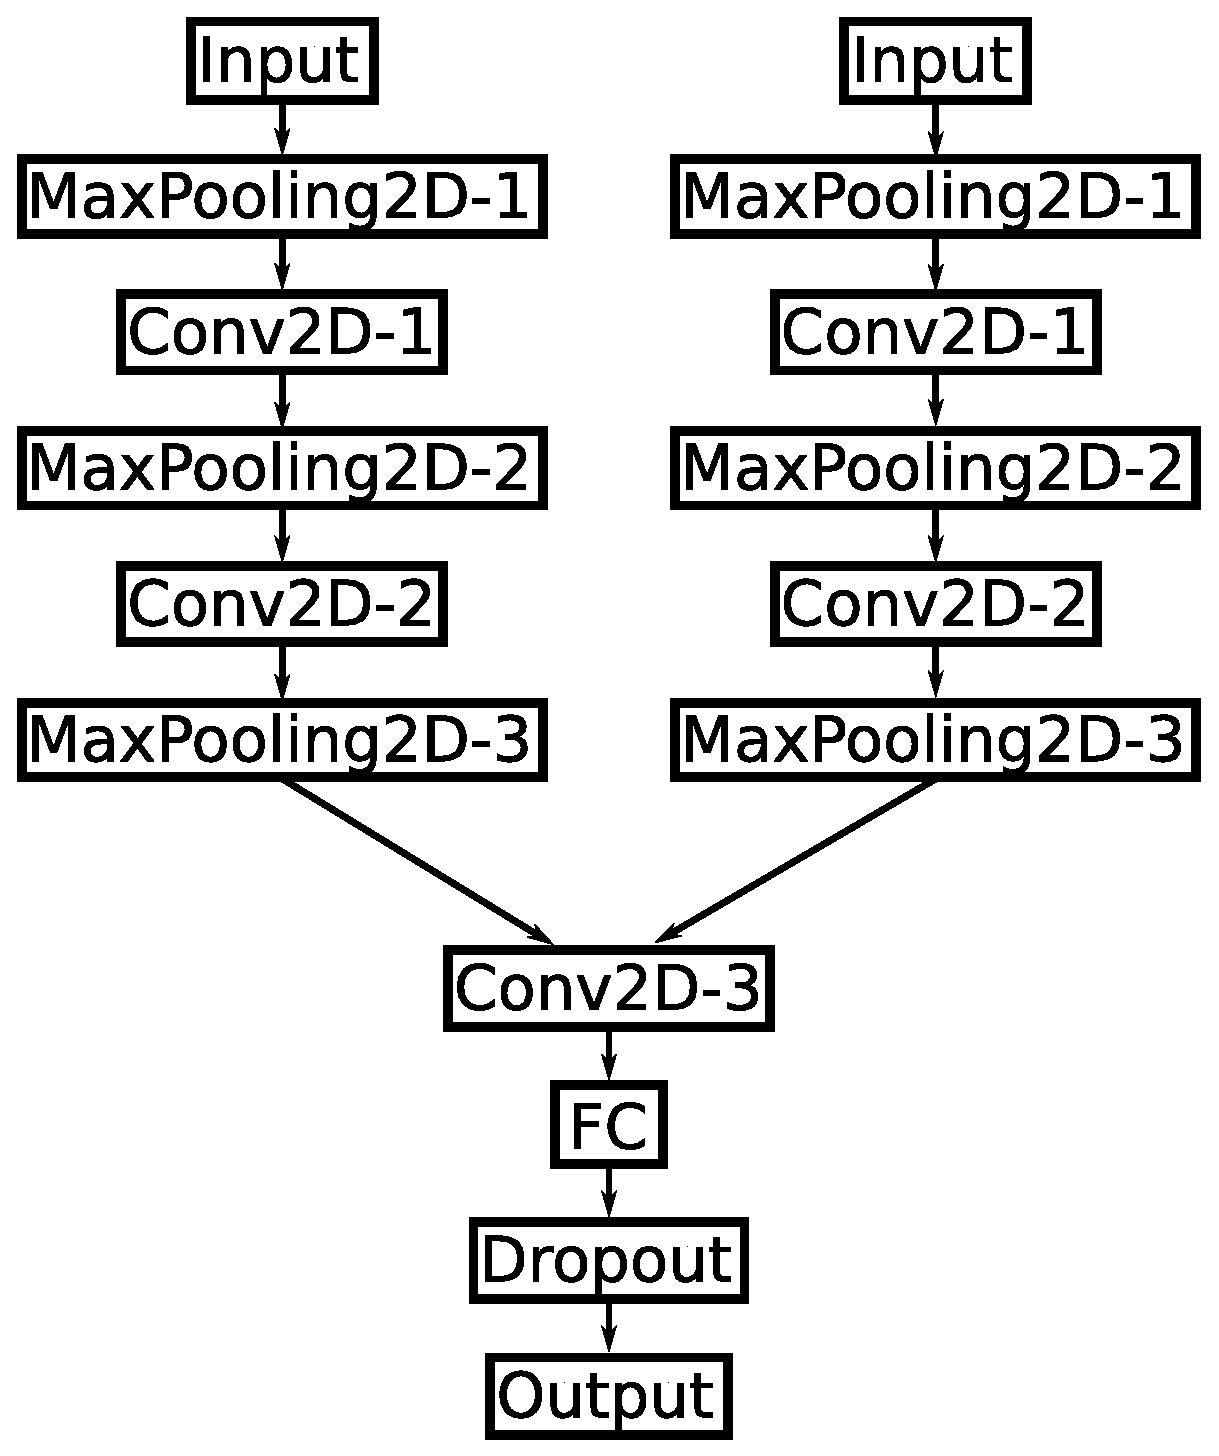
\includegraphics[clip, width=15zw]{eps/event_selection.eps}
  \caption{データの選別を行うためのニューラルネットワーク}
  \label{fig:selection}
\end{wrapfigure}

従来手法では識別に複雑な分岐条件が必要になるなどの問題点があった。
そこで、我々は近年注目されているニューラルネットワークを用いることで、
これらの問題点克服する新しい解析方法の開発を試みた。
ニューラルネットワークを用いることで、
離れた点の関係や直線の位置、角度などの従来の解析手法ではまとめて扱うことの難しい
多くの特徴量を同時に考慮した画像識別が可能になると期待される。
また、ニューラルネットワークは一度構築するとその後は短時間で画像識別を行うことができる。
このようなニューラルネットワークの特徴を活かすことで、
従来のアルゴリズムでは実現が難しかった高い精度と短い識別時間を実現することが可能である。

\begin{wrapfigure}{r}{15zw}
  \centering
  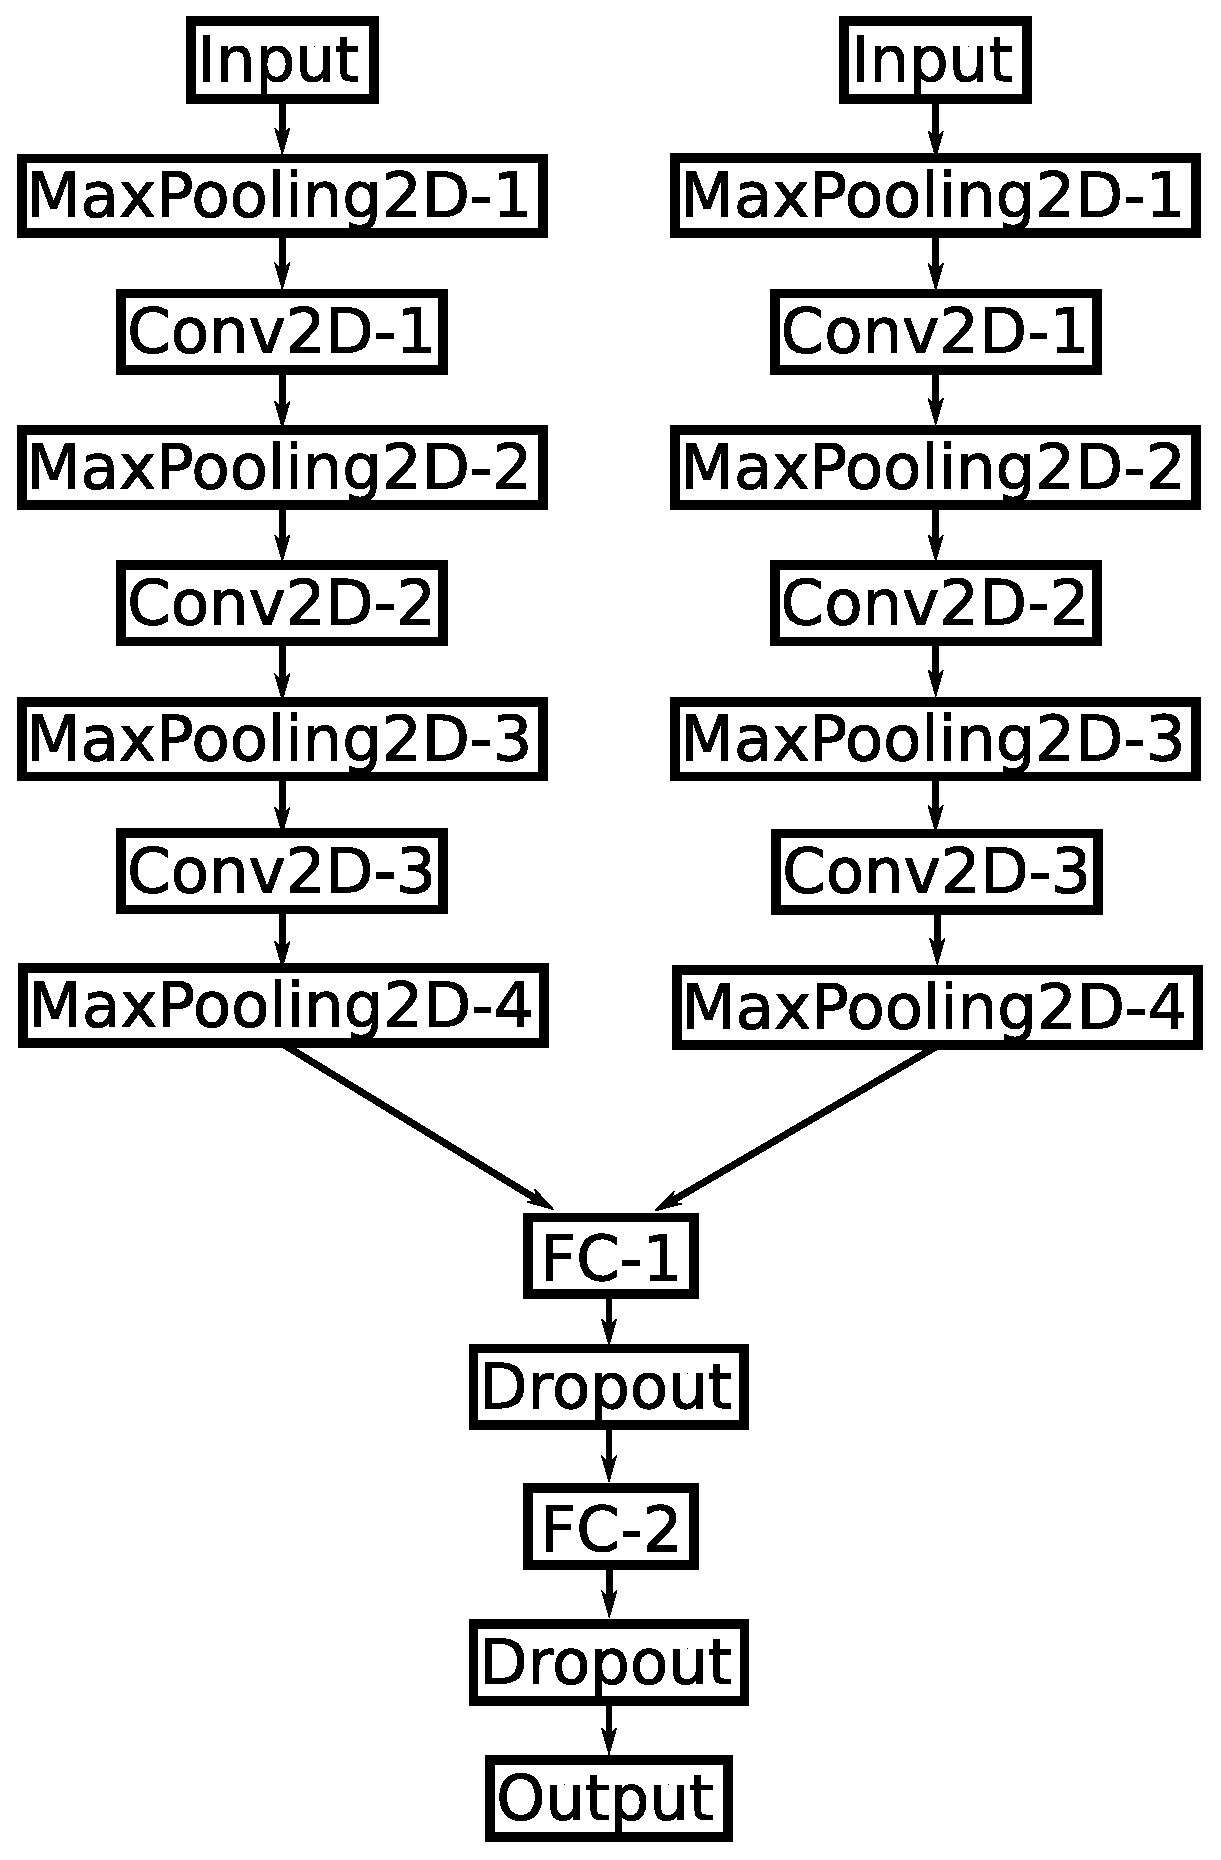
\includegraphics[clip, width=15zw]{eps/point_detection.eps}
  \caption{画像から情報を抽出するためのニューラルネットワーク}
  \label{fig:extraction}
\end{wrapfigure}

MAIKo TPC から得られるデータが画像であるため、画像認識に有用であるConvolutional Neural Network (CNN) を用いた。
CNN とはネットワーク内に畳み込み層を有するネットワーク構造である。
解析には事象の選別と軌跡情報の抽出の2つの段階があるため、
2種類のニューラルネットワークを用いて解析を行った。
事象の選別を行うニューラルネットワークと
画像から情報を抽出するニューラルネットワークの構造を
それぞれFig. \ref{fig:selection}とFig. \ref{fig:extraction}に示す。

事象選別のためのニュラルネットワークは、MAIKo TPC から得られる2つの平面に射影された飛跡画像を入力し、
その事象が標的と散乱した事象である確率を出力する。
出力された確率がある値以上である場合にその事象を標的と散乱した事象であると判断する。
このネットワークは16層からなり、2入力1出力の形をしている。
側面に射影した飛跡とビーム方向に射影した飛跡とでは画像の持つ意味が異なるため、
2つの入力が別れた構造を持つネットワークを構築した。
人間が判断したデータを用いて、学習および評価を行った。
学習には2,700 events、評価には300 events を使用した。

飛跡情報を抽出するためのネットワークは、MAIKo TPC から得られる2つの平面に射影された飛跡画像を入力し、
散乱が起こった座標と反跳した${}^{4}\rm{He}$が停止した座標を出力する。
学習を効率的に行うために、出力される座標は各軸が0--1の範囲になるように規格化した座標系で得られる。
このネットワークは21層からなり、2入力1出力の形をしている。
教師データには従来手法で決定した座標を用いた。
学習には3,012 events、評価には1,554 events を使用した。

学習環境はIntel Core i7、Nvidia GeForce GTX 1080Ti、Ubuntu 18.04 LTS、
TensorFlow~\cite{tensorflow}+Keras~\cite{keras} を用いた。

\section{Result}
選別のためのニューラルネットワークは、2,700 events に対して200 回学習を行った。
学習にはおよそ26分、その後の推測にはおよそ1秒かかった。
学習後の識別能力および学習過程をTable \ref{tab:result_selection}、
Fig. \ref{fig:history_selection}に示す。
各指標の定義は式 (\ref{eq:acc})--(\ref{eq:jac})、
各変数の意味はTable \ref{tab:variable}の通りである。
従来の手法と比較してすべての指標においてより高精度に選別が可能となった。
また、パラメータチューニングおよび選別に要する時間も大きく短縮することができた。

\begin{table}
  \begin{center}
  \caption{評価指標における変数の意味}
  \label{tab:variable}
    \begin{tabular}{|c|c|c|c|}
      \hline
      \multicolumn{2}{|c|}{} & \multicolumn{2}{c|}{\textgt{Judged by analysis}}\\ \cline{3-4}
      \multicolumn{2}{|c|}{} & Signal & Background \\ \hline
      \multirow{2}{*}{Eye-scanned} & Signal & SS & SB \\ \cline{2-4}
      & Background & BS & BB \\ \hline
    \end{tabular}
  \end{center}
\end{table}

\begin{align}
  \rm{Accuracy} &= \frac{\rm{SS}+\rm{BB}}{\rm{SS}+\rm{SB}+\rm{BS}+\rm{BB}} \label{eq:acc}\\
  \rm{Efficiency} &= \frac{\rm{SS}}{\rm{SS}+\rm{SB}}\\
  \rm{Purity} &= \frac{\rm{SS}}{\rm{SS}+\rm{BS}}\\
  \rm{Jaccard} &= \frac{\rm{SS}}{\rm{SS}+\rm{SB}+\rm{BS}} \label{eq:jac}
\end{align}

\begin{figure}
  \begin{minipage}{0.45\columnwidth}
    \centering
    \tblcaption{新手法の識別能力}
    \label{tab:result_selection}
    \begin{tabular}{lrr}
      \toprule
      index & Neural network (\%) & Hough (\%) \\ \midrule
      Accuracy & 96 & 89 \\
      Efficiency & 98 & 94 \\
      Purity & 94 & 84 \\
      Jaccard & 93 & 80 \\ \bottomrule
    \end{tabular}
  \end{minipage}
  \hfill
  \begin{minipage}{0.45\columnwidth}
    \centering
    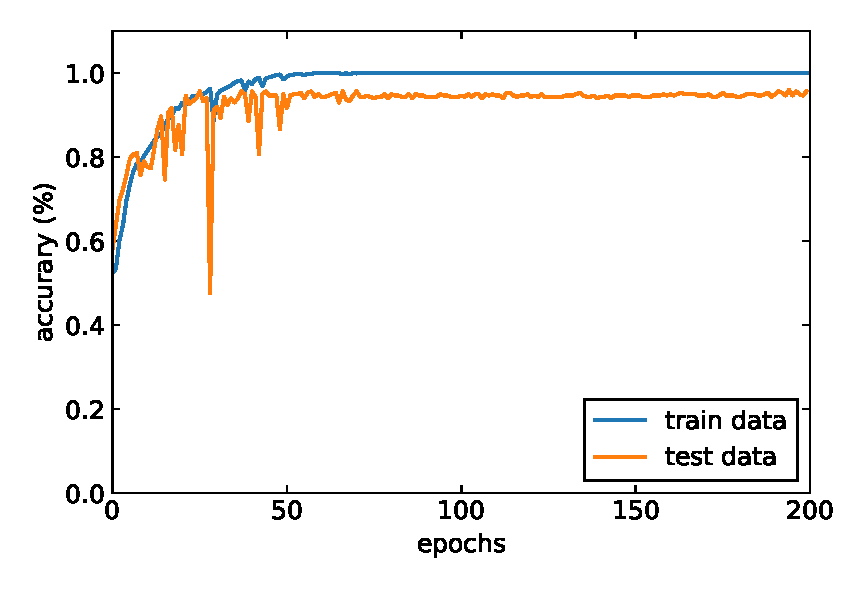
\includegraphics[clip,width=0.8\columnwidth]{eps/event_selection_history.eps}
    \caption{識別のためのニューラルネットワークの学習過程}
    \label{fig:history_selection}
  \end{minipage}
\end{figure}

座標の決定のためのニューラルネットワークは、3,012 events に対して500 回学習を行った。
学習にはおよそ270分、その後の推測にはおよそ2秒かかった。
学習後にニューラルネットワークが予測した座標と従来手法によって決定した座標の比較をFig. \ref{fig:result_detection} に示す。
学習過程をFig. \ref{fig:history_detection}に示す。
従来手法の精度を維持しつつ、
従来の手法と比較してパラメータチューニングおよび情報の抽出にかかる時間を短縮することができた。

\begin{figure}
  \centering
  \begin{minipage}{0.45\columnwidth}
    \centering
    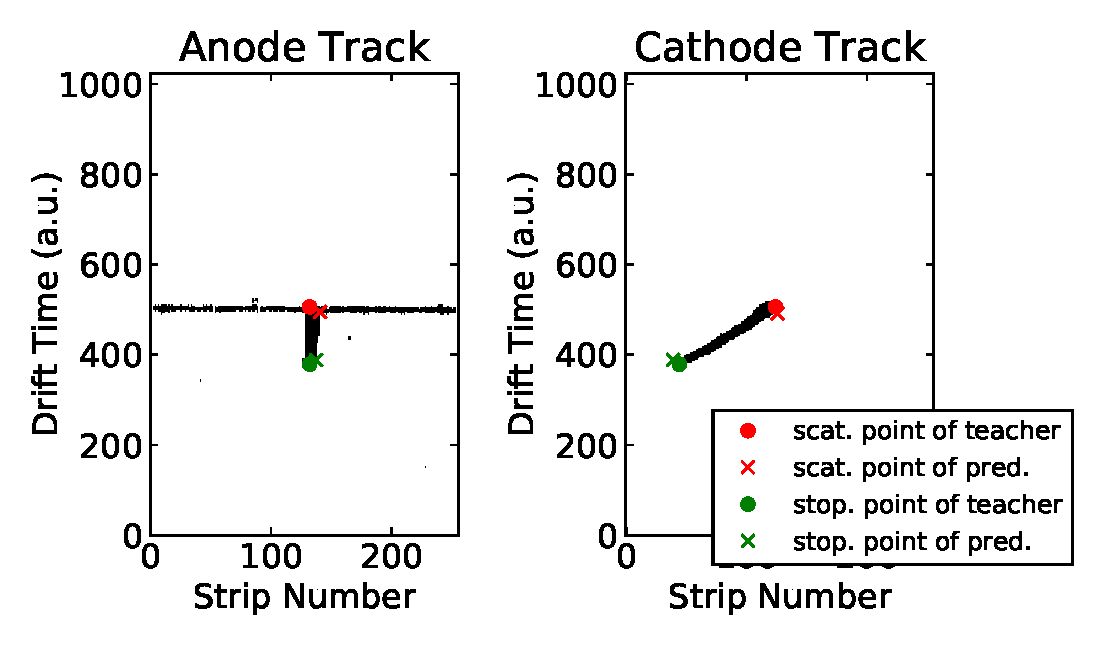
\includegraphics[clip,width=0.9\columnwidth]{eps/point_detection_compair.eps}
    \caption{ニューラルネットワークによって決定した座標とHough 変換によって決定した座標との比較}
    \label{fig:result_detection}
  \end{minipage}
  \hfill
  \begin{minipage}{0.45\columnwidth}
    \centering
    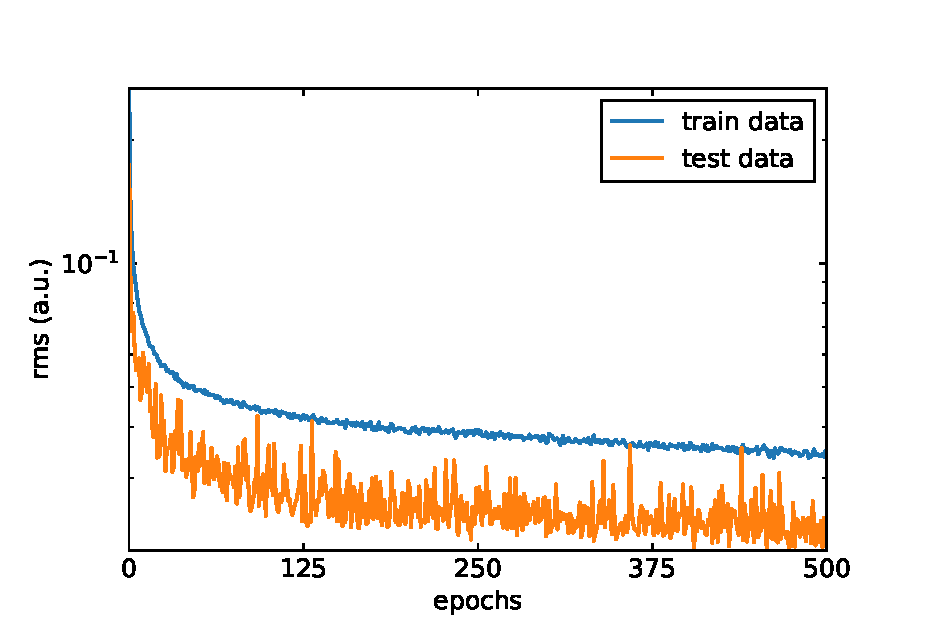
\includegraphics[clip,width=0.9\columnwidth]{eps/point_detection_history.eps}
    \caption{座標決定のためのニューラルネットワークの学習過程}
    \label{fig:history_detection}
  \end{minipage}
\end{figure}

\section{Conclusion}
従来のHough 変換を用いた画像識別アルゴリズムに変わる、
ニューラルネットワークを用いた新手法の開発を行った。
新手法は従来のものよりも高速かつ高精度に画像を識別することが可能となった。
また、飛跡情報の抽出については従来の精度を保ちつつ、高速に行うことが可能となった。
ニューラルネットワークを用いた解析手法はTPC の解析に有用であることがわかった。

\begin{thebibliography}{9}
\bibitem{mupic}
  A.~Ochi, T.~Nagayoshi, T.~Tanimori, T.~Nagae, and M.~Nakamura
  Nuclear Instruments and Methods in Physics Research A \textbf{471} 264 (2001)
\bibitem{MAIKo}
  T.~Furuno, T.~Kawabata, H.~Ong, S.~Adachi, Y.~Ayyad, T.~Baba, Y.~Fujikawa, T.~Hashimoto, K.~Inaba, Y.~Ishii,
  S.~Kabuki, H.~Kubo, Y.~Matsuda, Y.~Matsuoka, T.~Mizumoto, T.~Morimoto, M.~Murata, T.~Sawano, T.~Suzuki, A.~Takada,
  J.~Tanaka, I.~Tanihata, T.~Tanimori, D.~Tran, M-, Tsumura, and H.~Watanabe
  Nuclear Instruments and Methods in Physics Research A \textbf{908} 215 (2018)
\bibitem{tensorflow}
  A.~Davis, J.~Dean, M.~Devin, S.~Ghemawat, I.~Goodfellow, A.~Harp, G.~Irving,
  M.~Isard, Y.~Jia, R.~Jozefowicz, L.~Kaiser, M.~Kudlur, J.~Levenberg,
  D.~Man\'{e}, R.~Monga, S.~Moore, D.~Murray, C.~Olah, M.~Schuster, J.~Shlens,
  B.~Steiner, I.~Sutskever, K.~Talwar, P.~Tucker, V.~Vanhoucke, V.~Vasudevan,
  F.~Vi\'{e}gas, O.~Vinyals, P.~Warden, M.~Wattenberg, M.~Wicke, Y.~Yu, and
  X.~Zheng, (2015).
  \url{https://tensorflow.org}
\bibitem{keras}
  F.~Chollet, et al. (2015). \url{https://keras.io}

%\bibitem{cp} The abbreviation for JPS Conference Proceedings should be ``JPS Conf. Proc." in the reference list.
%\bibitem{jpsj} The abbreviation for the Journal of the Physical Society of Japan should be ``J. Phys. Soc. Jpn." in the reference list.
%\bibitem{ptep} The abbreviation for the Progress of Theoretical and Experimental Physics should be ``Prog. Theor. Exp. Phys." in the reference list.
%\bibitem{instructions} More abbreviations of journal titles are listed in ``Instructions for Preparation of Manuscript", which is available at our Web site (http://jpsj.jps.or.jp).
%\bibitem{format} F. Author, S. Author, and T. Author, Abbreviated journal title \textbf{volume in bold face}, initial page or article number (year of publication).
\end{thebibliography}

\end{document}

